\section{Catalog of real-time mitigation techniques}
\label{section:hardware:catalog}

\subsection{Existing real-time implementations}
\label{subsection:hardware:catalog:existing}
\subsubsection{Avoidance}
Most radio telescopes operate in an automated fashion, following a scheduler. The locations of known fixed sources of RFI, such as terrestrial emitters and geostationary satellites, are well-established. These fixed sources can be factored into the telescope's schedule, allowing for optimized observation strategies that minimize the impact of RFI on collected data. This is achieved by aligning the telescope's sequence of sky pointings with a model of its directivity pattern, avoiding these known interference sources.

In a more dynamic approach, the telescope can also avoid known moving sources of RFI, such as medium Earth orbit (MEO) satellites and aircraft. Satellite position data is publicly available, and aircraft locations can be tracked using ADS-B transmissions. However, avoiding low Earth orbit (LEO) satellites poses a greater challenge due to their high angular speeds and sheer numbers.

Dynamic interference avoidance strategies are being proposed for next-generation telescopes like FAST, ngVLA, and DSA-2000. ASKAP is also developing an RFI avoidance scheme to address atmospheric ducting events, which can channel RFI over large distances

\subsubsection{Adaptive analog attenuators}

The Owens Valley Radio Observatory Long Wavelength Array, in the US, employs adaptive attenuators to maintain stable baseline levels and prevent saturation in response to strong citizen broadcast RFI, which skips through the atmosphere during the day but not at night. Adaptive attenuators play a critical role in ensuring that the telescope array can handle this variable interference environment by dynamically adjusting the signal attenuation to counteract sudden increases in RFI or fluctuations arising from environmental factors like temperature, sky conditions, and antenna pointing. This approach effectively prevents saturation and preserves measurement accuracy, though it reduces sensitivity, limiting deep, sensitive observations to nighttime hours when the RFI is less intense. However, observations of particularly strong sources, such as the sun, remain unaffected by this daytime mitigation strategy, allowing these studies to proceed with minimal interference impact. By automating the attenuation adjustments, OVRO-LWA can continuously monitor the RFI environment and dynamically apply optimal gain settings, balancing the need to counteract interference with the goal of maximizing observational capabilities.

\subsubsection{Pre-LNA superconducting filters}
The current RFI mitigation framework at the Yebes Observatory, in Spain, utilizes hardware-based high-temperature superconducting (HTS) filters positioned ahead of the low-noise amplifiers. While effective, these filters present inherent limitations, including resonances or spurious responses at other frequencies within the receiver’s band. Moreover, as permanent components of the system, they cannot be automated. Recent advancements in filter design, such as the superconducting spiral bandpass filter developed by Huang et al. using a pseudo-Fourier technique, have demonstrated enhanced interference suppression capabilities \cite{huang2018superconducting}. Garcia-Carreno’s doctoral research further investigates optimization of cryogenic receivers using superconducting filters, addressing both RFI suppression and reference signal phase measurement \cite{huang2018superconducting}. Additional improvements are anticipated, with new filter designs currently under development and expected for publication.

\subsubsection{Front-end notch filters}

Strong narrowband RFI from various sources that affect the upgraded GMRT receiver’s dynamic range and linearity are mitigated using band reject/notch filters. These are incorporated in the front end of the receiver system to ensure that the system operates in the linear region by rejecting strong and persistent RFI from strong short-range transmissions, mobile communication, and broadcast television \cite{sureshkumar2016rfi}. Efforts to use the latest techniques to have the filter before the LNA are being developed to avoid saturation due to strong interfering signals.

\subsubsection{Switchable notch filters Green Bank}

The Green Bank Telescope (GBT) incorporates several advanced techniques for RFI mitigation, including the use of switchable notch filters, which are crucial for suppressing specific frequency bands prone to RFI contamination. In particular, within the C-band (4–8 GHz) receiver system, a notch filter is employed to attenuate interference from the 7.2075 GHz reference tone used in observations. This filter is positioned prior to the first amplifier in the C-band receiver chain, effectively reducing the amplification of the interfering signal and enhancing the clarity of astronomical data \cite{gbt1}. 

To further assist with RFI management, the GBT has also developed advanced tools that provide observers with real-time information on the RFI landscape. These resources include a graphical user interface (GUI) and an interactive web-based platform that allows users to access RFI scans and adjust their observational plans to avoid frequencies with significant interference. The combination of switchable notch filters and these proactive RFI monitoring tools substantially improves the GBT’s observational fidelity and data reliability.

\subsubsection{Digital: Excision in time}

\begin{itemize}
\item Real-time RFI Excision at GMRT

The upgraded GMRT (uGMRT) \cite{gupta2017upgraded} operates from 120 to 1450 MHz and has near-seamless coverage in this band. It is an array of 30, 45m diameter parabolic dishes and a sensitive receiver which operates in the interferometry and beamformer modes. The array is located 80 km north of Pune in India. The increase in the population around the array in the last 30 years along with the proliferation of communication devices, satellites, and mobile phones, has caused an increase in the RFI. The uGMRT signal processing backend has a real-time RFI excision system for mitigating RFI and achieving sensitivity levels close to the theoretical limits. \\

\begin{figure}
    \centering
    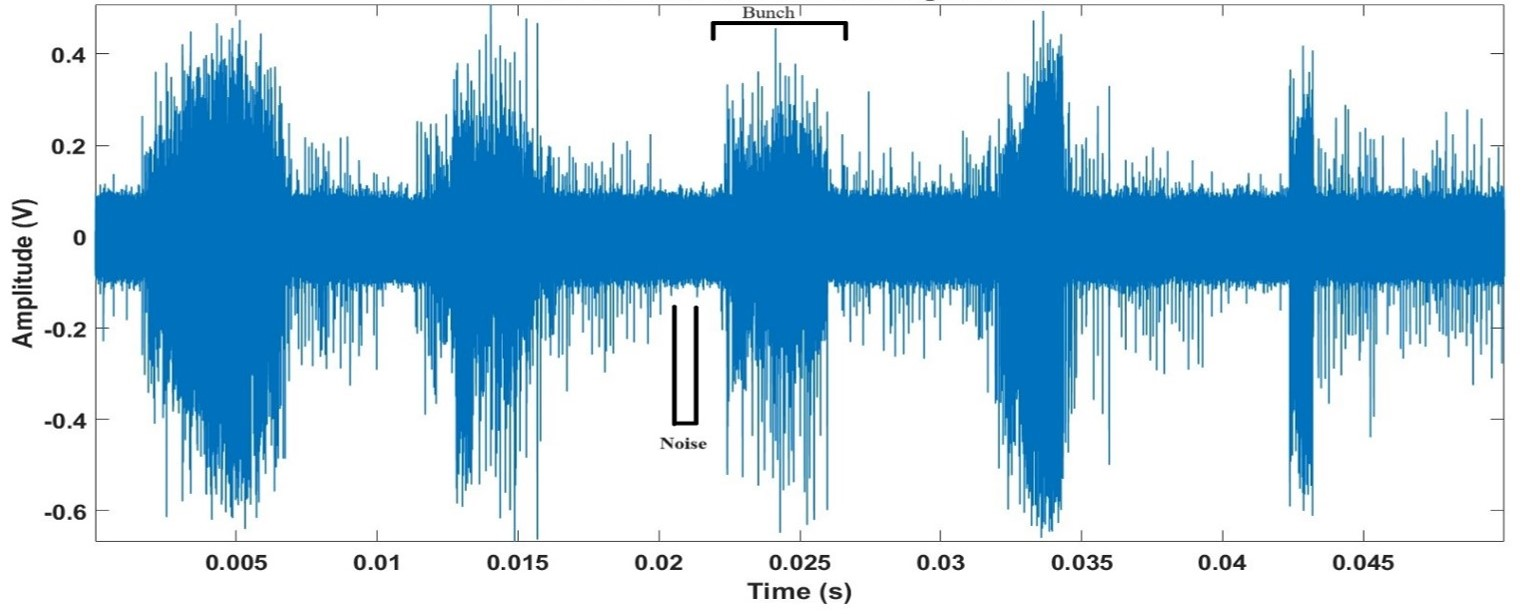
\includegraphics[scale=0.7]{Hardware Excision Techniques/figures/Band4_timeseries_ed.jpg}
    \caption{A 50ms time-series of single antenna Band-4 (550-850 MHz) data. Powerline RFI can be seen to occur in bunches repeating every 10ms. The data is acquired at the input of the signal processing system with a time resolution of 5ns.}
    \label{fig:ugmrt-b4-ts}
\end{figure}

One of the main causes of RFI at frequencies less than 1 GHz is sparking and corona discharge on the high-tension lines and transformer installations around the array. This type of RFI is impulsive in the time domain (Ref. Figure~\ref{fig:ugmrt-b4-ts}) resulting in a broadband increase in the power in the spectral domain. Since this type of RFI cannot be mitigated by frequency selective filters in the receiver system, a real-time statistical RFI excision system was developed which operates on digitized time-series from each antenna and polarization. This system is designed to excise strong impulses in the received signal. \\

The real-time system currently implemented on FPGA \cite{buch2019real} uses a median-based robust estimation and threshold detection scheme. Each incoming sample (at Nyquist rate) is compared with a robust threshold and samples detected as RFI are replaced with a constant value, threshold or digital noise sample. After rigorous testing on various astronomical data products, the RFI system is released for observations and is currently extensively used for observations in the lower frequency bands of uGMRT (< 1GHz). An example of imaging through this system wherein half the antennas used the original signal whereas the other half used the filtered copy \cite{buch2022performance} is shown in Figure~\ref{fig:ugmrt-b4-image}. \\

\begin{figure}
    %\centering
    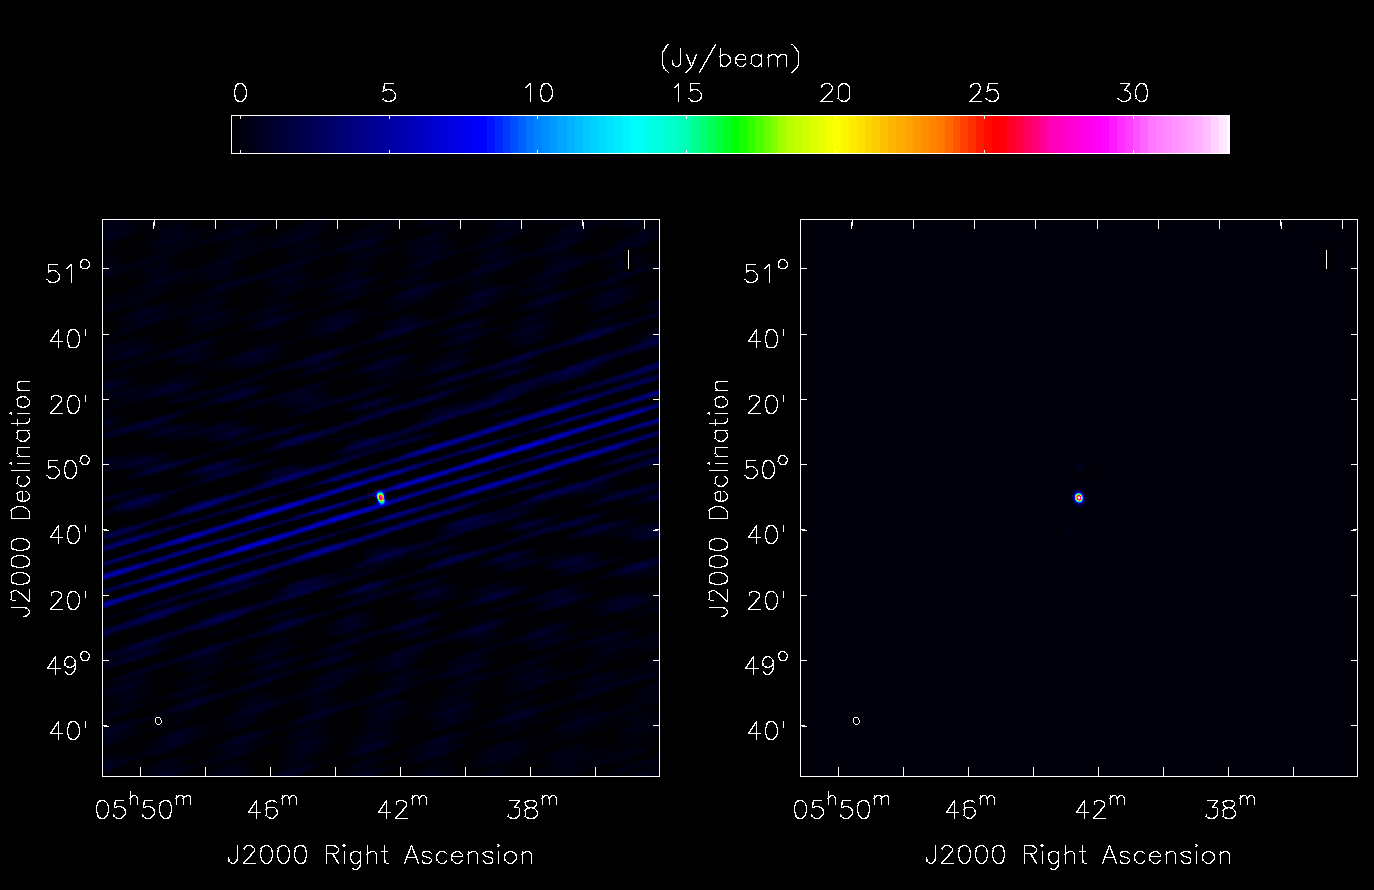
\includegraphics[scale=0.4]{Hardware Excision Techniques/figures/band4_point_source_rfi_filtering.png}
    \caption{uGMRT image, 9 antenna, point source 3C48 observed in band-4 (550-850 MHz). The image is built using baselines $<$0.5km and tested simultaneously to see the effects of real-time RFI filtering. The image corrupted by broadband RFI (left) is improved by a factor of 3 in the filtered version (right). Image courtesy: Ruta Kale, NCRA, India.
}
    \label{fig:ugmrt-b4-image}
\end{figure}

A possibility of refinements to the technique including mitigating low-level RFI, using learning-based approaches, and implementing similar techniques in real-time for mitigating narrowband RFI \cite{buch2016real} is being looked at. The technique is also being proposed \cite{buch2023real}for upcoming telescope like the SKA.\\


\item Post-channelization flagger\\
The DSA-2000 (Deep Synoptic Array 2000) is a next-generation radio telescope array designed to map the entire northern sky at high sensitivity, enabling unprecedented studies of transient phenomena and large-scale cosmic structure. Comprising 2,000 antennas spread across a large area, the DSA-2000 will provide continuous monitoring of the radio sky, particularly suited to detecting fast radio bursts and other dynamic cosmic events. The F-engine subsystem of the telescope manages key front-end processes, including signal conditioning through amplification and filtering, digitization, channelization, and packetization, enabling the transmission of raw data over a network to downstream processing nodes. As the only subsystem that receives the full processing bandwidth for each antenna, the F-engine is uniquely suited for identifying non-linearities that arise from harmonics or intermodulation products due to strong RFI. Detection of these non-linearities is achieved via two methods: high-cadence ($\approx$0.1 µs) monitoring of the total received power, compared to a calibrated operational range, and low-cadence ($\approx$0.1 s) assessment of spectral shape anomalies, based on root mean square differences between the integrated autocorrelation spectrum and a calibrated spectral model. Both binary detection mechanisms will be implemented, with a logical OR operation to combine them, producing a flag to indicate non-linear responses. This flag is subsequently passed to the X-engine, responsible for the antenna signal correlations, where visibility data from affected antennas is either statistically adapted at lower integration times or fully nulled, depending on the impact of the non-linearity.
\end{itemize}

\subsubsection{Digital: Excision in spectral}
\begin{itemize}
\item Sigma Cut real-time flagger

 RFIm \cite{sclocco2019real} is an open-source, high-performance library designed to mitigate RFI in real-time. RFIm is optimized to run on many-core accelerators such as GPUs and provides methods that are robust yet computationally efficient. The library features two main algorithms: Time-Domain Sigma Cut (TDSC) and Frequency-Domain Sigma Cut (FDSC). These two algorithms detect and replace RFI-contaminated data with statistical averages to reduce false positives without significant impact on processing time. This approach allows systems like the Apertif Radio Transient System (ARTS) to maintain high data throughput while effectively identifying real astronomical signals amidst increasing anthropogenic and satellite-generated interference.
 
\item Higher-order statistics

The Spectral Kurtosis (SK) technique is a statistical method used for real-time detection of non-Gaussian signals, such as radio frequency interference (RFI), within Gaussian noise in radio astronomy data. The SK estimator distinguishes signals by comparing power and power-squared values of spectral data to detect deviations from Gaussian behaviour. The Expanded Owens Valley Solar Array (EOVSA) implements this SK technique in its correlator, using an FPGA-based system to perform real-time SK calculations directly within the Fourier transform engine \cite{}. This design allows the system to flag and exclude contaminated data dynamically, enhancing the quality of observations by effectively identifying and mitigating RFI while preserving genuine astronomical signals.

\item MeFisTo: Frequency and Time Median filter on Nançay Decameter Array

Between 5 and 88 MHz, the lowest part of the frequency band accessible to ground-based telescopes, the sky is crowded with audio and timing broadcast users, allocated to frequency channels much closer than the frequency resolution required to meet the scientific needs of solar and Jovian observations. This band is also affected by wideband RFI generated by electric fences, spark ignition systems from internal combustion engines, and power lines.

Time and frequency analysis of this band must be performed with temporal and spectral resolutions far exceeding the requirements for scientific observations. This results in data streams and data sets much larger than necessary for scientific purposes.

Since 2013, a receiver \cite{lecacheux2013, 2017pre8.conf..455L} based on 80-MSps ADCs and a Stratix IV FPGA has implemented a real-time streaming Blackman-Harris-windowed 64k-FFT, followed by classical (averaged) time-frequency analysis using a Welch-averaged periodogram. Simultaneously, the same periodogram is computed with a median filter (kernel size=64) applied first on the frequency axis, then on the time axis (kernel size=128), to mitigate narrowband and wideband RFI in observations. The frequency resolution for RFI mitigation is as low as 1.2 kHz, but it is raised to 78 kHz for scientific purposes. The time resolution for RFI mitigation is 0.8 ms but is increased to 104 ms to provide a sustainable data rate for 24/7 monitoring of the Sun and Jupiter.

\begin{figure}[ht]
    \centering
    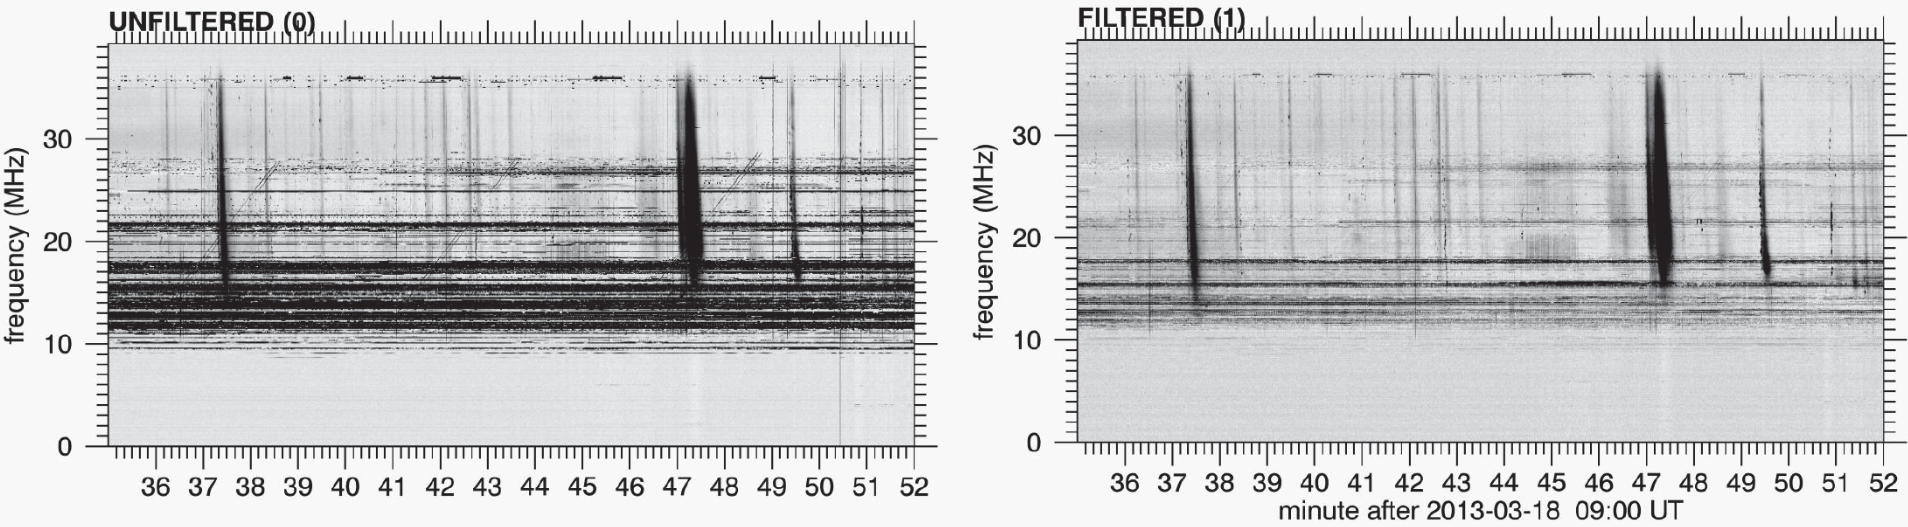
\includegraphics[width=\textwidth]{figures/MeFisTo.png}
    \caption{Solar activity observed without (left) and with (right) RFI median TF-filtering.  Wideband RFI and ionospheric sounders are eliminated, and shortwave broadcasts are significantly attenuated. \cite{lecacheux2013}}
    \label{fig:rfi_MeFisTo}
\end{figure}


\item Power-based excision RFI mitigation implementations at Nançay Observatory

In the early 20th century, a configurable digital receiver (RDH: Reconquest of Hertz Domain) was deployed at the Nançay Observatory. The receiver's ADC+FPGA+DSP system was shared by the 100-meter Decimeter Wavelength Telescope (NRT) and the Decameter Wavelength Analog Phased-Array (NDA). The main purpose of this receiver was to develop operational techniques for RFI mitigation. This hardware is now largely obsolete and was decommissioned years ago. However, the techniques remain and may be reused in future deployments.

The core work in designing these operational RFI mitigation techniques relies on a detailed study of the statistical behaviour of operators that can be easily implemented in real-time digital logic to create robust mean power estimators \cite{dumezviou:tel-00319939}. This toolbox can then be used to develop custom implementations that address the challenges encountered in the design of digital receivers for radio astronomy.  Next, two implementations are presented:

\begin{itemize}
\item HI red-shifted radio galaxies have the rest frequency of the hyperfine transition at 1420 MHz shifted into frequency bands allocated to L-band radar systems used for civil and military aircraft detection and ranging. Every 5 or 10 MHz, a radar system emits several kilowatts of power for one microsecond, with a pulse rate period of one millisecond. Theoretically, the sky is clear during the remaining 999 microseconds and available for astronomical observations. Detecting strong radar pulses with SNRs tens of dB above system noise is straightforward. The challenge lies in detecting weak pulses with negative-dB SNRs while maintaining an acceptable false alarm rate.

This was successfully implemented in the very limited resources of Virtex II FPGAs using the previously mentioned toolbox, allowing the excision of data blocks contaminated by both weak and strong radar pulses before they are passed to the spectral analysis block. As a result, HI surveys can now be conducted without artifacts originating from radar systems.


\item Red-shifted OH mega-masers may have their 1665 and 1667 MHz lines fall into the band the Iridium satellite constellation uses. This system manages access to the radio spectrum through a TFDMA scheme. During the test campaign, only a few percent of the millisecond-scale instantaneous spectrum was occupied, but after a few seconds of integration, the entire band became corrupted.

Spectral analysis was configured to generate data with time and frequency resolutions (3.4 kHz and 2.34 ms) tailored to the TFDMA characteristics. A MAD-estimated power criterion was then applied to discriminate between corrupted and pristine data slots, removing RFI from the dataset before integration.

\begin{figure}[ht]
    \centering
    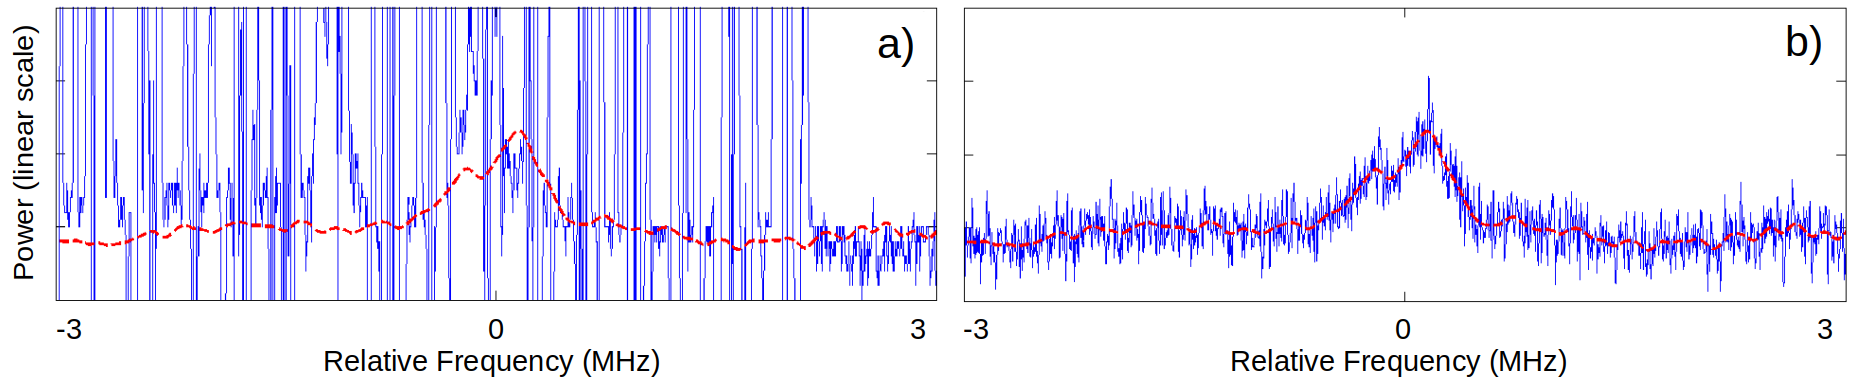
\includegraphics[width=\textwidth]{figures/IIIZw35_20040108.png}
    \caption{Re-observation of III Zw 35 on January 8, 2004, in real-time after 14 minutes of integration with the NRT: (a) Without "blanking." The vertical axis is adjusted to make the expected source profile visible. (b) With "blanking" (3.5\% of data eliminated). The source is visible again.}
    \label{fig:rfi_Iridium_blanked}
\end{figure}

This was implemented on TMS 6203 TI DSP chips to process the frequency band in real time.
\end{itemize}


\item CHIME: The Canadian Hydrogen Intensity Mapping Experiment \href{https://chime-experiment.ca/en}{(CHIME)} is a radio telescope primarily designed to study the distribution of neutral hydrogen gas in the Universe. Serendipitously, it turned out to be an excellent instrument for detecting fast radio bursts (FRBs), the mysterious millisecond-long radio flashes of unknown origin. When processed with the CHIME FRB pipeline, strong impulsive RFI may lead to false positives and therefore needs to be mitigated \cite{chime_frb_rfi_2023}. Several real-time iterative processes have been applied iteratively to weed out the statistical outliers from the channelized intensity data that are effectively high-pass filtered.

The RFI mitigation process before the dedispersion transform in L1-pipeline for CHIME/ FRB search is explained in \cite{chime_frb_rfi_2023}. The channelized intensity data of each beam are processed by 'subpipeline' containing alternate \textit{Clipping transforms} and \textit{Detrending transforms chains}. There are two different clipping transforms: intensity and standard deviation clipping transforms, to mask the statistical outliers in the intensity data. Every clipping iteration helps
improve the RFI mask by recognizing more statistical outliers and hence reshaping the masked intensity PDF to a robust $\chi^2$ distribution in real-time. The large-scale variations from RFI, forward gains, and digital beamforming are seen in the CHIME/FRB intensity time series as functions of the time, frequency, and sky location. Due to the distorted intensity PDF, the clipping and dedispersion transforms fail. The proposed detrending transforms provide a computationally less-intensive way of high-pass filtering in the harmonic space of intensity.

\item Correlator Outlier Excision
The MeerKAT correlator's initial data ingest stage employs a streamlined, one-dimensional mean absolute deviation (MAD) filter, termed “ingest\_rfi,” which operates along the frequency axis to independently threshold each data dump and correlation product. Implemented on a GPU, this filter is conservatively tuned to detect prominent amplitude spikes, flagging approximately 4\% of the L-band data for imaging modes, excluding pulsar observations, which are subject to a specialized RFI mitigation approach. Originally, flagged data from “ingest\_rfi” was excised before averaging the 0.5-second raw correlator dumps into the final 8-second dumps, though this was ultimately revised based on feedback from the scientific and RFI research communities. Currently, the “ingest\_rfi” flags are applied conservatively, while the more assertive “cal\_rfi” flags are typically excluded. Observers utilizing the MeerKAT pipeline images receive outputs with all standard flags applied. Further details can be found in the MeerKAT flagging package documentation \cite{hugo2022tricolouroptimizedsumthresholdflagger}.

\item Calibration VarThreshold
The calibration pipeline following the ingest stage at MeerKAT incorporates an advanced, two-dimensional RFI flagging algorithm, “cal\_rfi,” custom-developed in Numba as an adaptation of the AOFlagger. This algorithm identifies background noise across both time and frequency axes in two stages: an initial pass to establish a smooth baseline on unflagged data, followed by a sum-thresholding step. Flagging is selectively applied to HV and VH (cross-hand) polarizations, with the resulting flags extended to HH and VV data. During calibration, “cal\_rfi” flags are set before gain determination for the calibrator and reapplied after gain corrections on the target, enabling more stringent RFI rejection parameters. This procedure typically flags about 20\% of L-band data across all imaging modes, with pulsar modes exempted, as they employ a distinct RFI management strategy.


\end{itemize}

\subsection{Prospective real-time implementations}
\label{subsection:hardware:catalog:prospective}

\subsubsection{Preventive: Dynamic scheduler (Greg)}
Dynamic scheduling in radio telescopes is a crucial strategy for mitigating RFI by adapting observational plans based on real-time RFI conditions. By continuously monitoring the spectrum and adjusting observation times and frequencies accordingly, dynamic scheduling maximizes data quality and minimizes RFI impact. For example, the Green Bank Telescope (GBT) uses real-time RFI monitoring tools to adjust its observation schedule, avoiding heavily contaminated frequency bands and allowing observations to proceed in cleaner spectral windows. The MeerKAT telescope in South Africa similarly employs dynamic scheduling to shift its observational focus during periods of high RFI, such as those caused by local broadcasting or transient sources like aircraft. The approach ensures optimal use of telescope time, especially in areas where RFI varies frequently, by prioritizing observations of frequencies least affected by interference. This adaptive scheduling framework is particularly beneficial for detecting faint cosmic signals, as it helps preserve data integrity across a range of frequencies and time scales.

\subsubsection{Preventive: satellite avoidance at Green Bank}
Satellite boresight avoidance is a technique to prevent satellites from directly illuminating a telescope's primary observation direction. In experiments conducted by the Green Bank Telescope (GBT) with Starlink satellites, this technique was tested \cite{nhan2024spectrumcoexistencedemonstrationeffectiveness} by adjusting the satellite constellation's configuration based on real-time telescope pointing data and predicted satellite trajectories. This approach minimizes interference by dynamically coordinating telescope operations with satellite activities, such as emission control and beam steering. The process is facilitated by the Operational Data Sharing (ODS) system, an autonomous platform developed by the National Radio Astronomy Observatory (NRAO). ODS provides satellite operators with real-time updates on telescope positions and observing frequencies, allowing them to adjust satellite operations accordingly. With frequent updates, potentially every minute, ODS ensures effective coordination, especially during close satellite passes near the telescope’s boresight

%\subsubsection{Analog: Notch filters for uGMRT (Kaushal)}
\subsubsection{Analog : Tunable notch filter DSA-2000 (Greg)}

The tunable notch filters are designed to mitigate RFI in the analog front end of the DSA-2000 receivers. The Quad-Stub Resonator Filter uses four high-Q “series LC” stubs, each controlled by voltage-tuned varactors, allowing independent frequency tuning for precise RFI mitigation. The filter achieves deep notch attenuation, adjustable within a range of 550 MHz to 1050 MHz, with peak attenuation up to 62.5 dB. It features a chassis design with RFI-tight seals and SMA connectors to prevent interference coupling. The filter's response is fine-tuned through individual varactor bias adjustments, enabling adaptable and effective RFI suppression across a broad frequency range.

\subsubsection{Analog: Reconfigurable Intelligent Surface (Greg)}

Reconfigurable Intelligent Surfaces (RIS) can mitigate RFI at the telescope receiver by dynamically shaping the electromagnetic wavefronts to create a destructive interference zone around the receiver \cite{zou2022scisrs,wei2024ris,wei2023multistage}. The RIS array, composed of multiple controllable elements, adjusts the phase and amplitude of reflected signals to precisely counteract incoming RFI. By steering reflected signals from the RIS in such a way that they are out of phase with the incident RFI, the RIS effectively cancels the RFI energy before it reaches the telescope’s receiver. This approach allows for the creation of an electromagnetic quiet zone, enabling the telescope to perform sensitive astronomical observations without interference from external RFI sources, such as aircraft and satellites, without altering the telescope’s primary astronomical signals.

\subsubsection{Digital: SK EDD Effelsberg}
The Effelsberg Direct Digitisation (EDD) System is a state-of-the-art fully digital receiver. Analog-to-digital conversion occurs directly in the frontend and the digital baseband signal is transmitted over 100-GbE Ethernet to a processing cluster, where the signal is fed into GPUs based on commodity off-the-shelf (COTS) components. While this approach requires extra effort to shield the receiver inputs from self-generated RFI from the extra hardware close to the receivers, it offers a lot of benefits in terms of signal quality and flexibility. Currently, there are several Pulsar, spectroscopy, spectro-polarimetry and VLBI modes available. Adding new features is easy owing to the versatility of the GPU approach. First tests are also ongoing to implement the spectral kurtosis estimator-based RFI flagging. 

\subsubsection{Digital: cyclic spectroscopy Green Bank}

The Green Bank Telescope (GBT) is actively developing a cyclic spectroscopy system aimed at high-resolution studies of pulsars and improving RFI mitigation. Cyclic spectroscopy is particularly valuable for separating the periodic signals of pulsars from RFI, allowing the system to maintain detailed phase and frequency resolution. This technique enhances the GBT’s ability to study narrowband interstellar scintillation structures and scattering delays, which can be distorted by RFI. By accurately capturing the cyclic structure of pulsar signals, cyclic spectroscopy helps distinguish astronomical signals from interfering sources like satellite transmissions, which lack this periodicity.

Moreover, cyclic spectroscopy at the GBT is complemented by other RFI mitigation techniques, such as spectral kurtosis, which monitors departures from Gaussian noise to identify RFI-contaminated data segments. This approach has proven effective across different astronomical sources observed at GBT, improving data quality by flagging and replacing RFI with representative noise, thus preserving the integrity of the scientific data collected.

\subsubsection{Digital: Excision in time parametric subtraction Ellingson (Greg)}

The time-domain coherent cancellation (CTC) technique is a method used to mitigate RFI by subtracting an interference estimate from the received signal in real-time \cite{ellingson2022coherent}. CTC operates by generating a reference signal that represents the interfering source, which can be acquired externally (e.g., through a separate antenna) or synthesized internally using prior knowledge of the interference. The reference signal is used to create an interference estimate that is coherently subtracted from the received signal, ideally leaving only the astronomical signal of interest with minimal added noise or distortion. The approach allows telescopes to "look through" interference, preserving affected data that would otherwise be discarded by traditional methods, though it requires precise estimation and synchronization to avoid errors that could compromise the scientific data.

\subsubsection{Digital: Threshold-based pre-correlation RFI detection technique to be used in SKA.Mid (Thushara)}
\label{subsection:hardware:catalog:ska-mid}

The Correlator Beamformer for the Mid-frequency telescope for the \href{https://www.skao.int/en}{Square Kilometre Array} (SKA-Mid.CBF) uses a 'power threshold-based' RFI detection scheme \cite{ska_mid_cbf_rfi_2019}. The main objective is to preserve the linearity of the signal chain while achieving the desired dynamic range to maintain the sensitivity. The architecture of the proposed RFI detector/flagger module is shown in Figure~\ref{fig:rfi_df_ska_mid_cbf}. As shown there, two time scales are involved:
\begin{enumerate}
    \item Long-term ($>$1 sec, considering on/off state of the noise diode) for establishing an average power level, and
    \item Short-term to detect and flag bursting RFI to prevent downstream spectral splatter.
\end{enumerate}

The number of samples used for the short-term power calculation is programmable. If the short-term power calculation is greater than a programmable threshold, set by the Telescope-Manage or internally determined if “auto-set”, then a flag is set and carried with the data stream to the downstream processing module, and downstream operations (i.e. any that affect output data products or intermediate calculations needed such as gains/levels settings) are inhibited for the number of samples that it takes the flag to propagate through all downstream processing modules. As per the flagging policy, both polarization components are flagged if one is flagged. The dwell time of the flag is also programmable to balance the data loss with the risk of contamination. Note that the flagged data is not used in evaluating the long-term power calculation to have an estimate of the signal level of the non-RFI-contaminated signal. The long-term power is accumulated in two separate bins, one for noise diode on, and one for noise diode off.

\begin{figure}
    \centering
    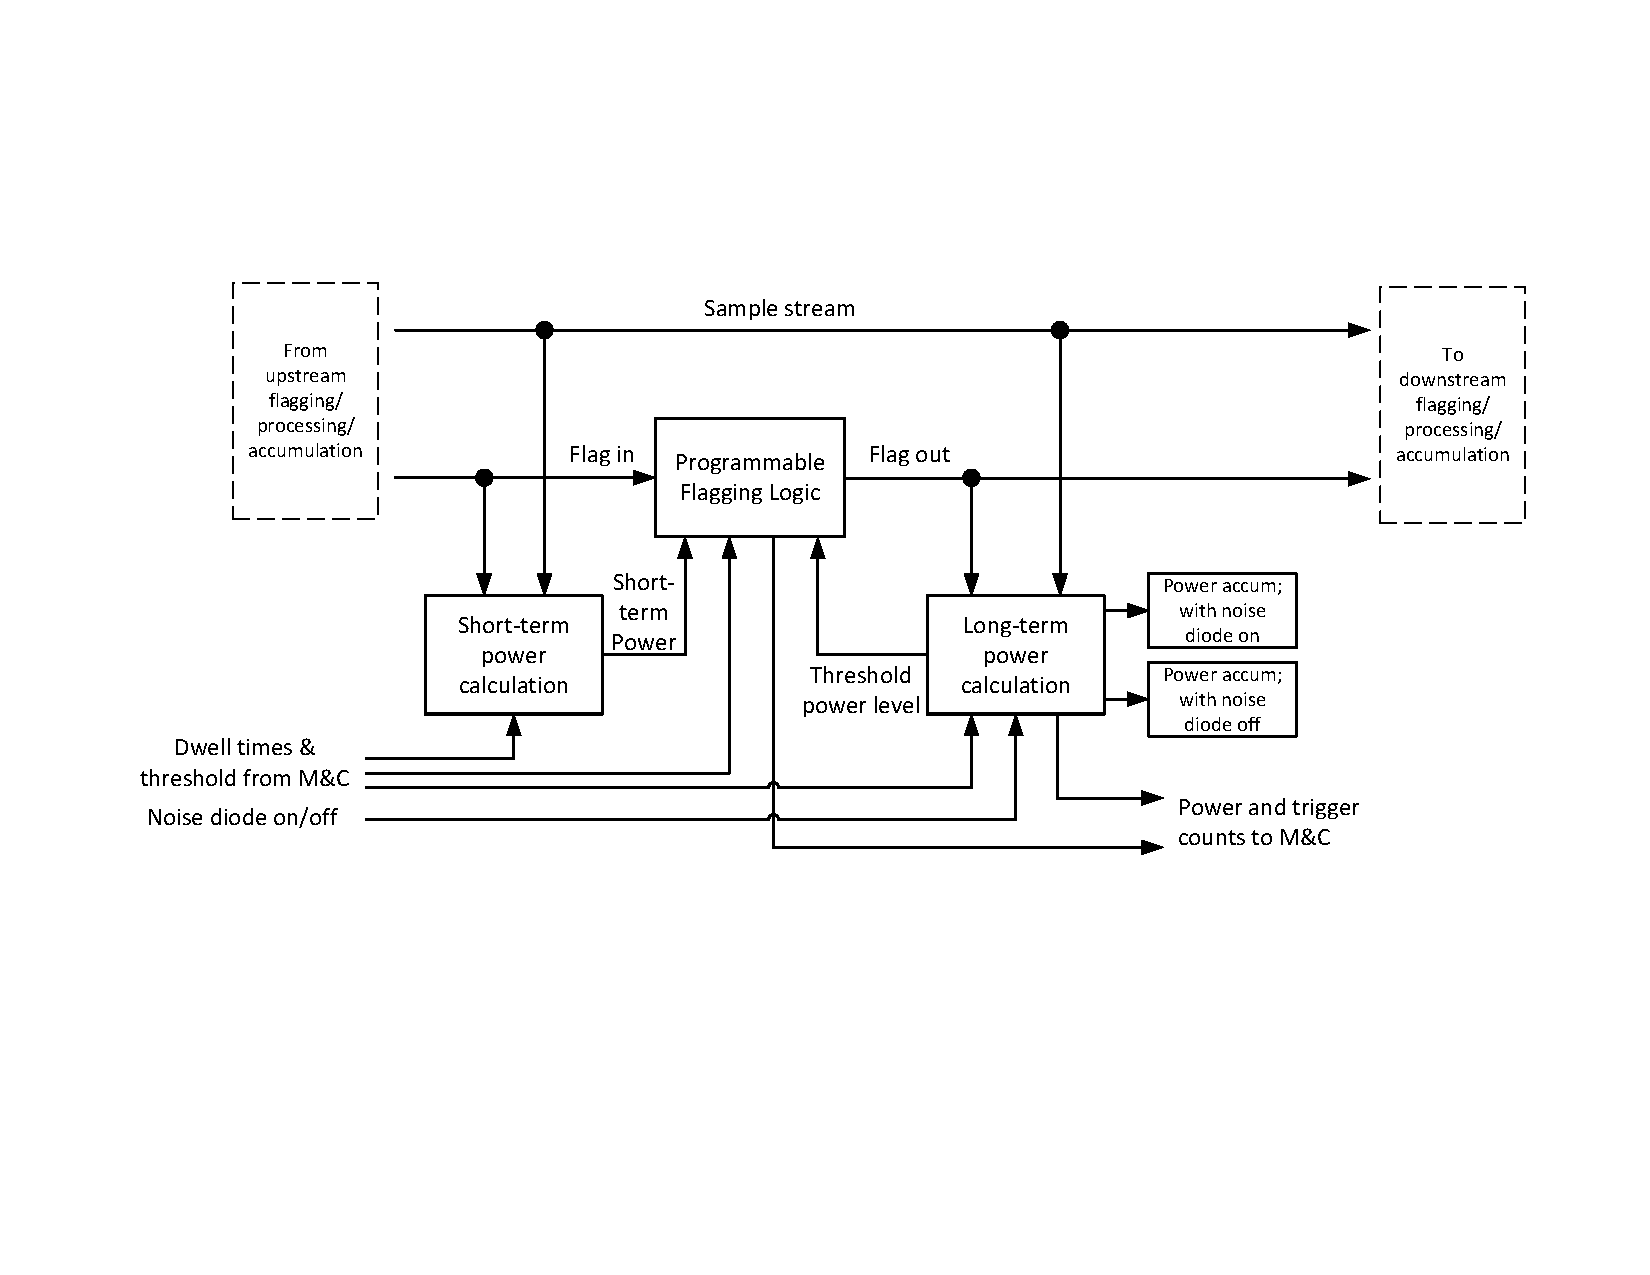
\includegraphics[height=.28\textheight]{figures/RFI_DF_SKA_Mid_CBF.pdf}
    \caption{The proposed RFI threshold detector/flagger (from \cite{ska_mid_cbf_rfi_2019}).}
    \label{fig:rfi_df_ska_mid_cbf}
\end{figure}


\subsubsection{Digital: excision in UV domain (Greg)}

GRIDflag \cite{10464448} is a UV-plane-based RFI flagging algorithm designed to enhance the sensitivity and imaging fidelity of radio interferometric observations in the presence of strong and persistent RFI. Unlike traditional methods that flag RFI in the time-channel plane of baselines, GRIDflag operates directly in the UV plane, where multiple baselines sample similar spatial Fourier components redundantly across a regular grid. By statistically comparing UV samples within each grid pixel, GRIDflag identifies and flags RFI-affected points, preserving UV coverage and sensitivity to spatial scales. This approach is particularly effective in mitigating systematic noise introduced by faint RFI, which can otherwise degrade image sensitivity and accuracy. GRIDflag's design allows it to be computationally efficient and adaptable to modern technologies like GPUs, making it well-suited for current and next-generation radio telescopes.

\subsubsection{Digital: Spatial filtering (Greg, Kaushal)}
\begin{itemize}
\item Classic spatial filtering

The core idea is to leverage the spatial diversity of RFI and astronomical signals, along with the unique spatial signatures of interfering sources, to separate and suppress RFI \cite{hellbourg2014radio,hellbourg2016spatial,hellbourg2014rfi}. By estimating the RFI subspace using techniques like Singular Value Decomposition (SVD) and exploiting cyclostationary properties of RFI signals, spatial filters are designed to project received signals onto subspaces orthogonal to the RFI, effectively nulling interference. These filters can be applied either before or after correlation stages in the data processing chain. The technique is particularly valuable for modern radio telescopes, such as LOFAR and EMBRACE, where dense antenna arrays provide numerous redundant measurements, enhancing the precision of RFI mitigation without significantly impacting the desired astronomical signal. This approach helps maintain high fidelity and sensitivity in observations despite increasing RFI challenges from human-made sources.

\item Reference-antenna

A reference antenna can be used to mitigate RFI in real time by providing an accurate estimation of the RFI spatial signature, which can then be used for spatial filtering in radio astronomy. The reference antenna is positioned to specifically capture the RFI without significantly receiving the astronomical signals. This RFI reference signal is correlated with the signals received by the main telescope array, allowing the RFI's spatial signature to be extracted and identified. This information is then used to project out the RFI from the main array's data using spatial filtering techniques, such as subspace projection.

By continuously updating the RFI spatial signature using subspace tracking algorithms, like the Power Method or Rayleigh Quotient Iteration, the system can adapt to changes in the RFI environment in real time, effectively cancelling out the interference without impacting the astronomical signals. This approach is particularly effective for managing multiple RFI sources and dynamically changing interference patterns, enabling high-fidelity observations even in heavily contaminated radio bands\cite{hellbourg2014reference,sardarabadi2015spatial}.

\end{itemize}
\subsubsection{Digital AI/ML} (Greg, Kaushal)
\begin{itemize}
\item Collaborative Signal Subtraction (Greg)

The collaborative approach to RFI mitigation works by establishing a bidirectional communication between radio telescopes and interfering sources, such as cellular networks, to actively share RFI information and cancel interference in real time. The interfering sources decompose their signals into a compact representation using techniques like the Karhunen–Loève Transform (KLT), which captures the signal's statistical properties independent of time and frequency. This RFI information, including eigenfunctions representing the interference, is periodically shared with the telescope through a low-overhead communication channel.

At the telescope, the received composite signal, which includes both astronomical signals and RFI, is similarly decomposed. The shared RFI characteristics are then used to cancel the interference from the telescope’s data through orthogonal projections in the eigenspace, thereby revealing clean astronomical signals. This approach significantly reduces communication and computational overhead by prioritizing the sharing of high-impact RFI data and selectively updating the interference model based on its influence on the telescope, thus maintaining high accuracy in signal recovery while managing multiple RFI sources effectively \cite{chakraborty2023collaboration,chakraborty2024low}.

\item Pattern recognition (Greg)

Automated pattern recognition to identify RFI in real-time radio astronomy data \cite{Winkel_2007} uses edge detection and window fitting to isolate high-intensity regions in the time-frequency domain, likely corresponding to RFI. Statistical analysis then helps differentiate RFI from genuine astronomical signals by comparing intensity patterns and variations. Iterative baseline fitting further refines the detection to ensure that RFI is accurately identified without impacting the integrity of the astronomical data. This method can be implemented in real-time systems, enabling dynamic flagging and mitigation of RFI, which is crucial for maintaining data quality in environments prone to interference, such as those near populated areas or satellite systems.

\item External flag generation (RFI monitor?) (Greg)

An RFI detector can provide real-time flags for radio telescopes by using machine learning techniques to automatically identify and classify interference in the radio frequency spectrum. The system described here \cite{9111666} employs a deep neural network (DNN) that processes time-frequency data, detecting and drawing bounding boxes around RFI events. This approach allows the detector to continuously monitor the RF environment and flag novel or anomalous RFI events in real time. The detected RFI events are flagged based on their spatial, spectral, and temporal characteristics, allowing the telescope to dynamically adjust its data processing pipeline to exclude or compensate for contaminated signals.

By integrating with the telescope’s data stream, the system can provide immediate notifications about RFI, enabling telescopes to respond promptly to interference without manual intervention. This real-time detection capability is particularly useful for maintaining the quality of astronomical observations by preventing the degradation of data due to unwanted interference.

\item Real-time RFI Prediction for Satellite RFI at GMRT

For spatially confined sources of interference that affect the GMRT for a fraction of the observing time when the beam of the telescope cuts the beam of the satellites, a real-time satellite monitoring system has been implemented. This system informs the user ahead of time about the satellite passes, and typical duration, logs the data, and raises an alarm in the control room \cite{raybole2016real}.

%\item Use of higher order statistics (Kaushal)
\end{itemize}

\subsubsection{System: The Sample Frequency Offset Sampling (Thushara)}

The pioneering Sample Frequency Offset Sampling method offers a systematic approach to mitigate the impact of strong out-of-band RFI contaminating the observed spectrum \cite{carlson_scfo_2017}. The Corelator Beamformer of Square Kilometre Array Mid Telescope (SKA Mid.CBF), is the first radio telescope to implement this method \cite{ska_mid_cbf_rfi_2019}. This method can also reduce the impact of artefacts generated in connection with the sample clock signals. 

In the proposed method for Sample Clock Frequency Offset (SCFO) sampling, each receptor in SKA1\_Mid is sampled at different sample rates, causing the strong RFI to leak into different Frequency Slices (FSs) at different frequencies. As a result, when cross-correlated, the leaked RFI components decorrelate based on the integration time and frequency offset. Additionally, the 'Shift-Resample-Shift-Back' method is used to mitigate the impact of strong RFI with high time occupancy that is concentrated in frequency bands (e.g., GSM, Digital-TV, and GNSS). This method takes advantage of the Frequency Slice Architecture in Mid.CBF, where each FS processes an approximately 200 MHz portion of the observing band. The FSs are shifted to position the strong RFI near the 0 Hz mark and then resampled to correct for SCFO sampling and delay-tracking, before being shifted back to their original frequency sense. While resampling with a 'fractional-delay filter-bank' introduces systematic sample-time jitters that create replicas of the input spectrum, adding a random delay-jitter can suppress these replicas at the cost of increasing the system's noise floor. However, the added noise power is directly related to the magnitude of the resampling error. By relocating the strong RFI close to the 0 Hz mark, the absolute error due to resampling is minimized, resulting in a lower system noise floor.